% Technical milestones; periods are not exclusive eras.
% Figure labels use single spacing, independently of the thesis body text.
\begingroup
\linespread{1}\selectfont
\begin{tikzpicture}[
  titletext/.style={font=\bfseries},
  subtitle/.style={font=\small\itshape, align=center},
  date/.style={font=\small, text=black!70, align=center},
  labeltext/.style={font=\small\bfseries, align=center, text width=3.4cm, inner sep=0pt},
  detail/.style={font=\footnotesize, align=center, text width=3.4cm, inner sep=0pt},
  imgnode/.style={inner sep=0pt, draw=black!35, line width=0.6pt},
  timeline/.style={-{Latex[length=2mm,width=1.4mm]}, thick, black!55},
  arr/.style={-{Latex[length=1.5mm,width=1mm]}, thick, steelblue31119180!70!black},
]
\begin{scope}[yshift=6.18cm]
\node[titletext] at (5.85,-5.88) {Technical progress};
\node[subtitle] at (5.85,-6.45) {building increasingly capable embodied visual systems};
\draw[timeline] (-1.55,-7.53) -- (13.25,-7.53);
\foreach \x/\era in {0/{1960s--1970s},3.9/{1980s--2000s},7.8/2010s,11.7/2020s} {
  \node[date] at (\x,-7.16) {\era};
  \fill[black!55] (\x,-7.53) circle[radius=1.6pt];
}
% The next three illustrations reuse one scene so the development of its
% representation, rather than a change of subject, is visually explicit.
\foreach \x in {0,3.9,7.8,11.7} {
  \filldraw[fill=black!2,draw=black!35,line width=0.6pt]
    (\x-1.6,-10.493) rectangle (\x+1.6,-7.827);
}
% Schematic input/output, not a recorded result from a historical algorithm.
% The wireframe uses the block dimensions and camera pose of history_scene.js.
\begin{scope}[shift={(0,-9.16)}]
  \node[inner sep=0pt] at (-0.87,0.42)
    {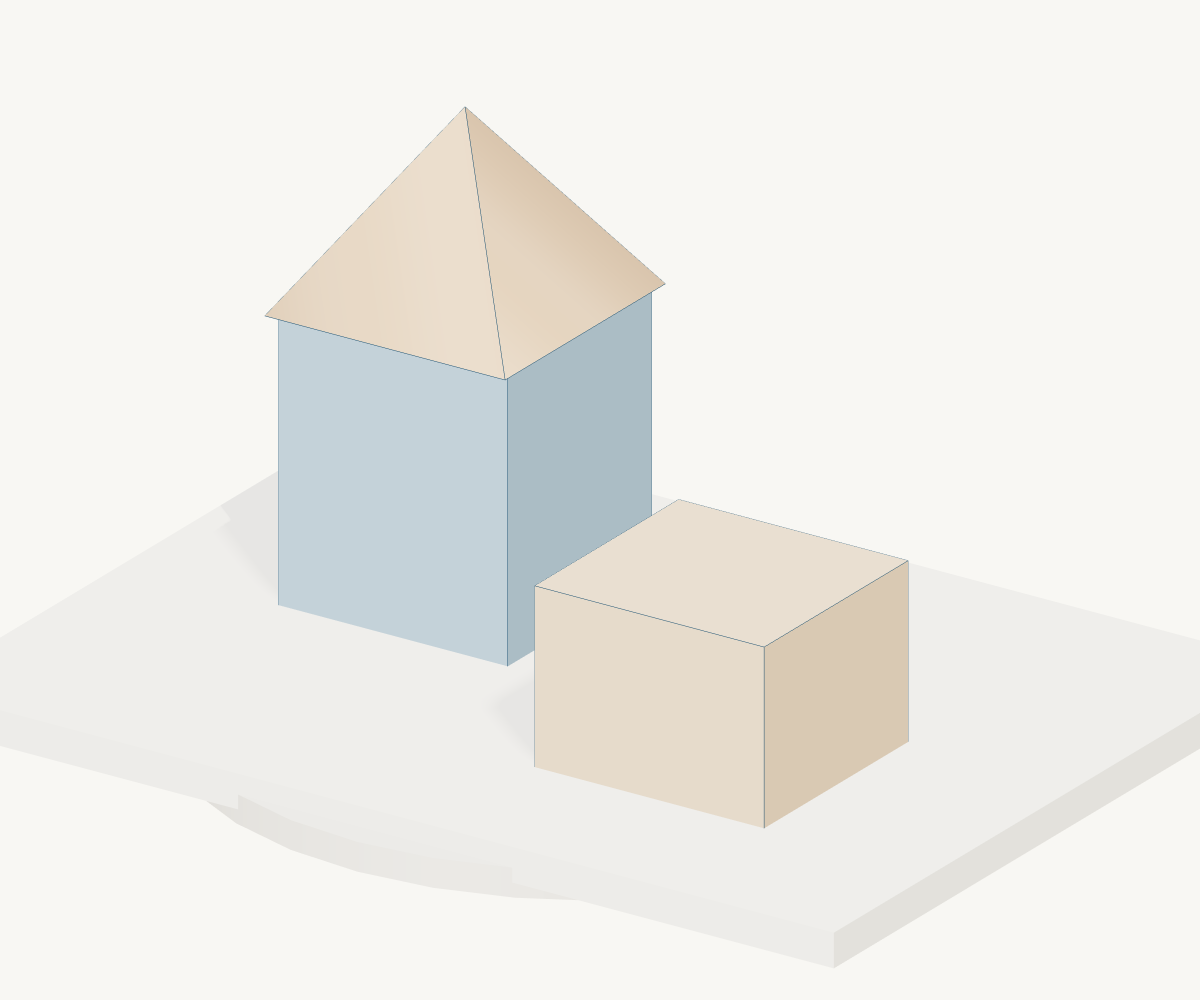
\includegraphics[width=1.30cm]{figures/img/main/three/renders/history_blocks.png}};
  \draw[arr] (-0.14,0.42) -- (0.15,0.42);
  % Orthographic basis for eye=(4,3.8,6), lookAt=(0,0.65,0), width=3.7.
  % Match the input's projection; the output omits the platform and shading.
  \begin{scope}[shift={(0.85,0.211)},
    x={(0.2923cm,-0.0780cm)},
    y={(0cm,0.3220cm)},
    z={(-0.1949cm,-0.1170cm)},
    visibleedge/.style={draw=steelblue31119180!85!black,line width=0.65pt},
    hiddenedge/.style={draw=black!35,line width=0.35pt,densely dashed}]
    \foreach \cx/\cy/\cz/\w/\h/\d in {-0.7/0.55/-0.3/0.85/1.0/0.8,0.65/0.36/0.30/0.85/0.62/0.80} {
      \begin{scope}[shift={(\cx,\cy,\cz)}]
        \coordinate (a) at ({-\w/2},{-\h/2},{-\d/2});
        \coordinate (b) at ({\w/2},{-\h/2},{-\d/2});
        \coordinate (c) at ({\w/2},{-\h/2},{\d/2});
        \coordinate (d) at ({-\w/2},{-\h/2},{\d/2});
        \coordinate (e) at ({-\w/2},{\h/2},{-\d/2});
        \coordinate (f) at ({\w/2},{\h/2},{-\d/2});
        \coordinate (g) at ({\w/2},{\h/2},{\d/2});
        \coordinate (h) at ({-\w/2},{\h/2},{\d/2});
        \draw[hiddenedge] (b) -- (a) -- (d) (a) -- (e);
        \draw[visibleedge] (b) -- (c) -- (d) -- (h) -- (e) -- (f) -- (g) -- (h)
          (b) -- (f) (c) -- (g);
        \foreach \v in {b,c,d,e,f,g,h}
          \fill[steelblue31119180!85!black] (\v) circle[radius=0.6pt];
      \end{scope}
    }
    % Four-sided roof: apex and base corners match the rendered pyramid.
    \coordinate (apex) at (-0.7,1.695,-0.3);
    \foreach \x/\z in {-1.145/-0.745,-0.255/-0.745,-0.255/0.145,-1.145/0.145} {
      \draw[visibleedge] (\x,1.045,\z) -- (apex);
    }
    \fill[steelblue31119180!85!black] (apex) circle[radius=0.7pt];
  \end{scope}
  \node[font=\scriptsize,align=center,text width=1.35cm] at (-0.87,-0.40) {image};
  \node[font=\scriptsize,align=center,text width=1.45cm] at (0.83,-0.40) {edges and\\vertices};
  \node[font=\scriptsize,draw=black!45,fill=white,rounded corners=1.5pt,
    align=center,text width=2.55cm,inner sep=4pt] at (0,-1.03) {3D structure};
\end{scope}

% Hand-crafted features: one local patch produces an illustrative histogram.
% This is a schematic descriptor, not a measured output of a named algorithm.
\begin{scope}[shift={(3.9,-9.16)}]
  \node[inner sep=0pt] at (-0.87,0.52)
    {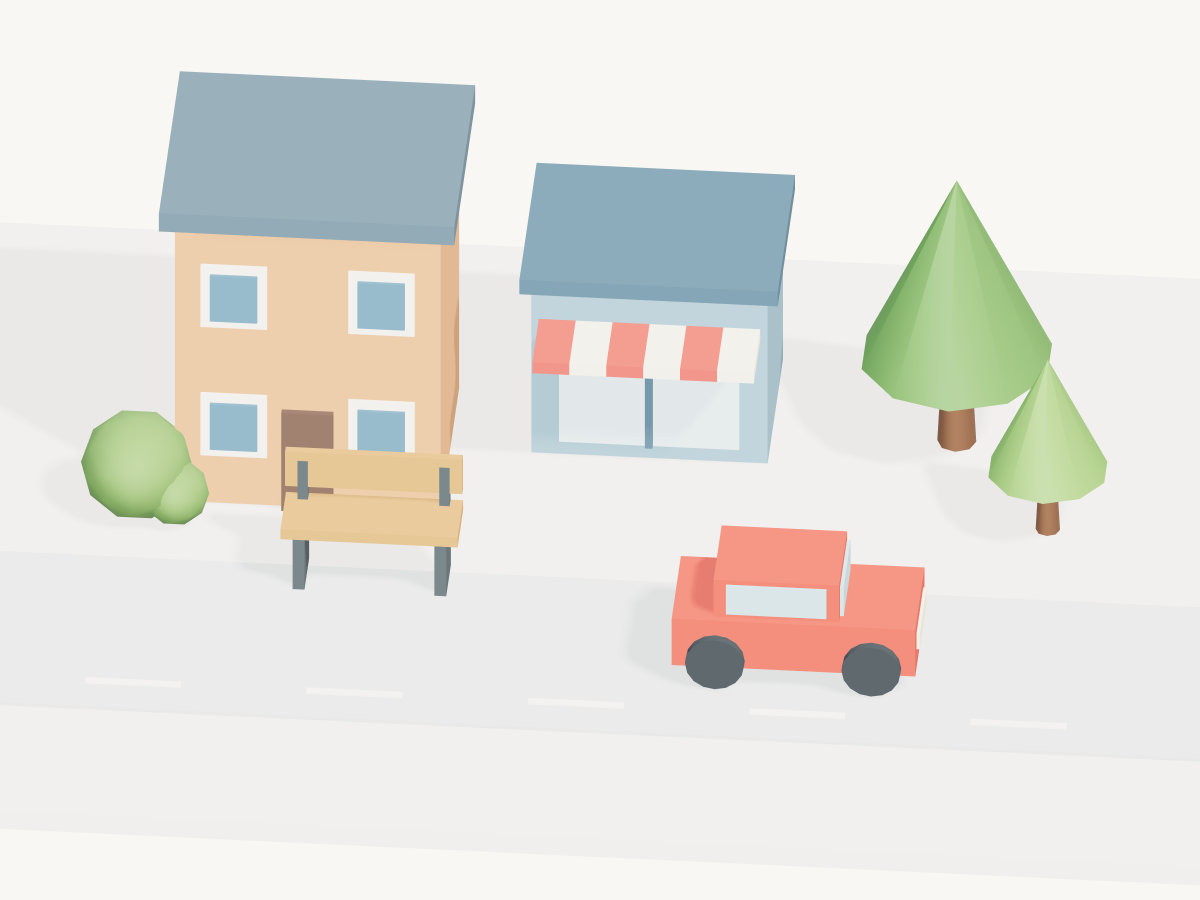
\includegraphics[width=1.30cm]{figures/img/main/three/renders/contributions_scene.png}};
  \draw[steelblue31119180!85!black,line width=0.8pt]
    (-1.30,0.50) rectangle ++(0.34,0.34);
  \draw[arr] (-0.14,0.52) -- (0.15,0.52);
  % Uniform bin widths and spacing keep the output readable at print size.
  \draw[black!45,line width=0.4pt] (0.24,0.20) -- (1.39,0.20);
  \foreach \i/\h in {0/0.18,1/0.34,2/0.55,3/0.40,4/0.23,5/0.12,6/0.28} {
    \fill[steelblue31119180!65] ({0.27+0.16*\i},0.20) rectangle ++(0.10,\h);
  }
  \node[font=\scriptsize,align=center,text width=1.35cm] at (-0.87,-0.20) {local patch};
  \node[font=\scriptsize,align=center,text width=1.45cm] at (0.83,-0.20) {gradient\\histogram};
  \node[font=\scriptsize,draw=black!45,fill=white,rounded corners=1.5pt,
    align=center,text width=2.55cm,inner sep=4pt] at (0,-1.03) {feature descriptor};
\end{scope}
% Convolutional feature maps: image -> learned hierarchy -> prediction.
\begin{scope}[shift={(7.8,-9.16)}]
  \node[inner sep=0pt] at (-0.86,0.60)
    {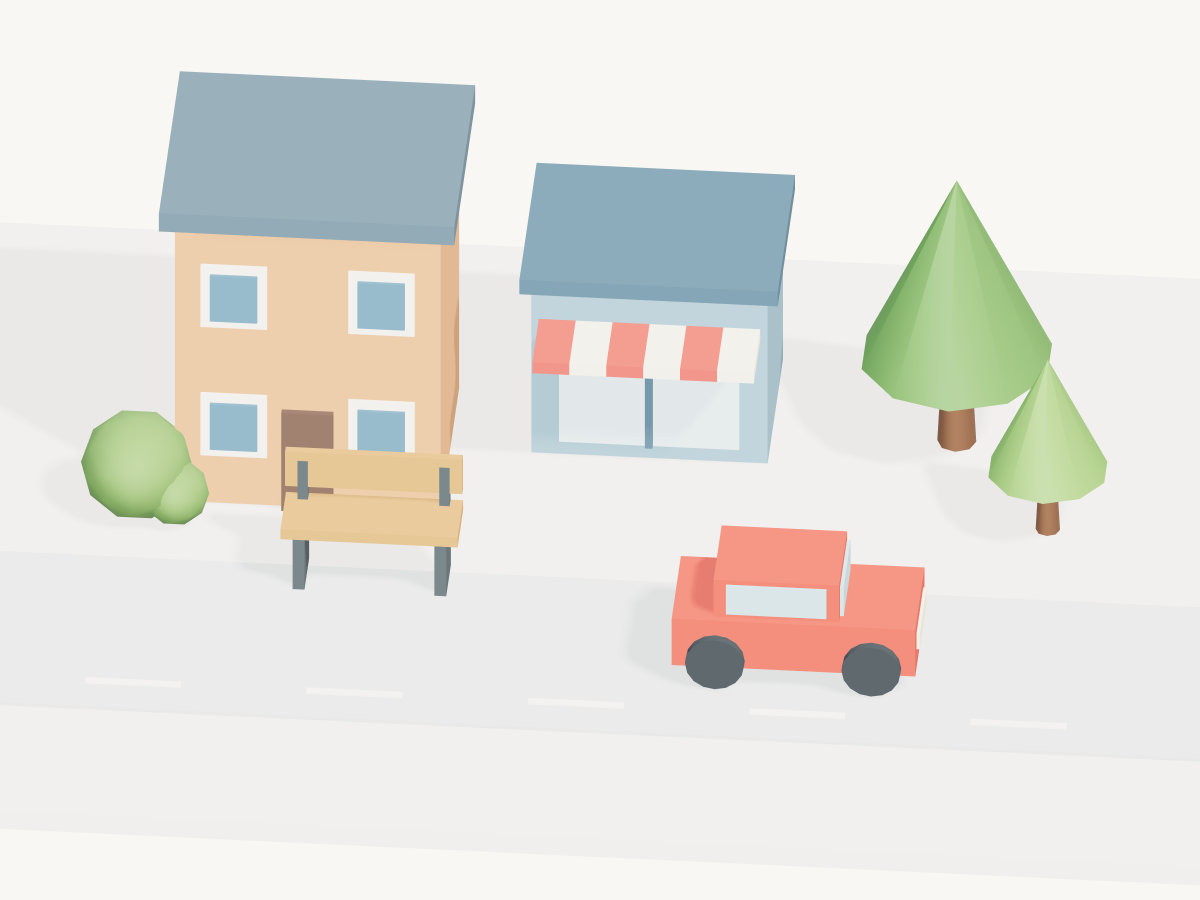
\includegraphics[width=1.08cm]{figures/img/main/three/renders/contributions_scene.png}};
  \draw[arr] (-0.25,0.60) -- (0.12,0.60);
  % Equal horizontal pitch and a gradual reduction in feature-map size.
  \foreach \i in {0,...,5} {
    \pgfmathsetmacro{\x}{0.20+0.20*\i}
    \pgfmathsetmacro{\h}{0.82-0.09*\i}
    \filldraw[draw=steelblue31119180!70!black,fill=steelblue31119180!20,line width=0.4pt]
      (\x,{0.60-\h/2}) -- ++(0.09,0.08) -- ++(0,\h) -- ++(-0.09,-0.08) -- cycle;
  }
  \node[font=\scriptsize,align=center] at (0,-0.15) {learned feature hierarchy};
  \draw[arr] (0,-0.40) -- (0,-0.71);
  \node[font=\scriptsize,draw=black!45,fill=white,rounded corners=1.5pt,
    align=center,text width=2.55cm,inner sep=4pt] at (0,-0.99) {predicted label: car};
\end{scope}
% Patch encoding and multimodal output, with no claim about a specific model.
\begin{scope}[shift={(11.7,-9.16)}]
  \node[inner sep=0pt] at (-0.80,0.65)
    {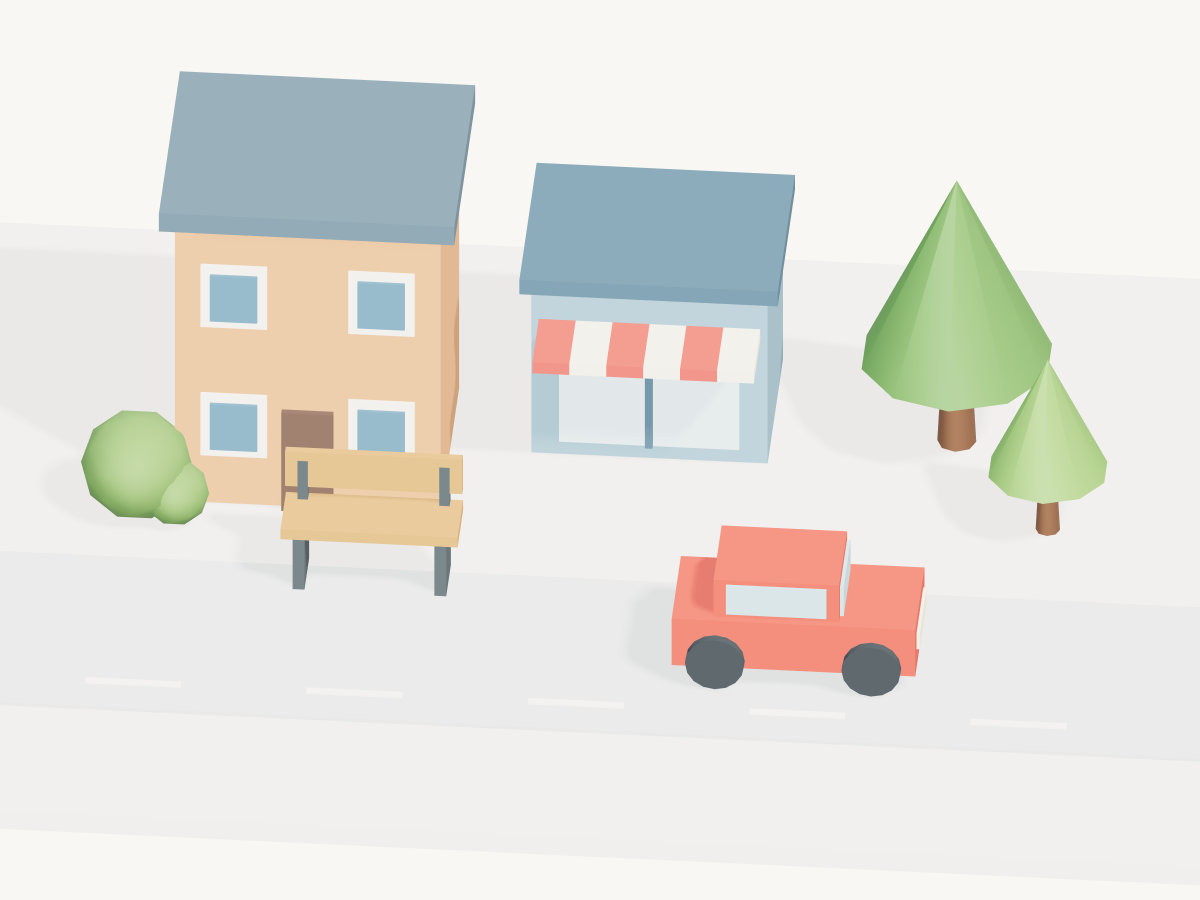
\includegraphics[width=1.08cm]{figures/img/main/three/renders/contributions_scene.png}};
  \draw[step=0.27,black!65,line width=0.3pt,shift={(-1.34,0.245)}] (0,0) grid (1.08,0.81);
  \draw[arr] (-0.17,0.65) -- (0.12,0.65);
  \node[draw=steelblue31119180!70!black,fill=steelblue31119180!10,
    font=\scriptsize,align=center,rounded corners=1.5pt,minimum height=0.65cm] (encoder) at (0.72,0.65) {multimodal\\model};
  \draw[arr] (encoder.south) -- (0.72,-0.20) -- (0,-0.20) -- (0,-0.41);
  \node[draw=black!45,fill=white,rounded corners=1.5pt,font=\scriptsize,
    align=center,text width=2.42cm,inner sep=4pt] at (0,-0.85) {text output:\\a street scene};
\end{scope}
\node[labeltext,anchor=north] (technicallabel1) at (0,-10.873) {Geometry and early\\machine vision};
\node[labeltext,anchor=north] (technicallabel2) at (3.9,-10.873) {Hand-crafted\\representations};
\node[labeltext,anchor=north] (technicallabel3) at (7.8,-10.873) {Deep visual\\learning};
\node[labeltext,anchor=north,text width=3.8cm] (technicallabel4) at (11.7,-10.873) {Foundation and\\vision-language models};
% Embodied-vision developments share the technical axis and the top panel's
% heading/example hierarchy, without a separate timeline or repeated dates.
\node[fit=(technicallabel1)(technicallabel2)(technicallabel3)(technicallabel4),inner sep=0pt] (technicallabels) {};
\node[detail,anchor=north] at ($(technicallabel1.center |- technicallabels.south)+(0,-0.25)$) {Early vision-guided robots};
\node[detail,anchor=north] at ($(technicallabel2.center |- technicallabels.south)+(0,-0.25)$) {Active and animate vision};
\node[detail,anchor=north] at ($(technicallabel3.center |- technicallabels.south)+(0,-0.25)$) {Learned visual attention};
\node[detail,anchor=north] at ($(technicallabel4.center |- technicallabels.south)+(0,-0.25)$) {Embodied exploration};
\end{scope}
\end{tikzpicture}
\endgroup
